%%%%%%%%%%%%%%%%%%%%%%%%%%%%%%%%%%%%%%%%%%%%%%%%%%%%%%%%
%GRASS PROMOTION FLYER                                 %
%(c) 2007 GRASS PROMOTION TEAM                         %
%GNU Free Documentation License                        %
%Version 1.2                                           %
%Needs leaflet.cls				       %
%www.ctan.org/tex-archive/macros/latex/contrib/leaflet/%
%%%%%%%%%%%%%%%%%%%%%%%%%%%%%%%%%%%%%%%%%%%%%%%%%%%%%%%%

%Sometimes printing engines need the 2nd side upside down
%in this case, use tumble (which is default) instead of notumble
%If this causes problems, use notumble
%If you need a foldmark, delete nofoldmark
\documentclass[notumble,a4paper,10pt,nofoldmark]{leaflet}
\usepackage{helvet,courier,xcolor}

% Set Helvetica as the default font
\renewcommand*\familydefault\sfdefault
% Let LaTeX knows that pictures are found in ./pix
\graphicspath{{pix/}}

% Setting up things for the captions
\usepackage{caption}[2004/07/16]
\captionsetup{%
  font={small,it},%
  labelformat=empty,% Leaves out label: ``Figure 1''
  labelsep=none,%
  aboveskip=0pt%
}
% Defining a new 'figure' environment for the document
\newenvironment{myfig}[1][0pt plus 1.5ex minus .5ex]{\par\vspace*{#1}\begin{minipage}{\textwidth}\centering}{\end{minipage}}

% Defining the GRASS homepage
\newcommand{\GRASSurl}{\url{http://grass.osgeo.org}}

% Define a color for the URIs
\definecolor{darkblue}{RGB}{0,0,88}

\usepackage{hyperref}
% Setting up some document info
\hypersetup{%
  colorlinks=true,%
  urlcolor=darkblue,% Redefine this color to change URIs color
  pdfauthor={A comunidade de GRASS},%
  pdftitle={SIG GRASS - Efici\^{e}ncia em liberdade \& transparencia -},%
  pdfsubject={GRASS Flyer promocional},%
  breaklinks=true,%
  plainpages=false%
}

% Title page stuff
\title{\textbf{\huge SIG GRASS}\\%
\textsl{Efici\^{e}ncia em liberdade \& transparencia}}
\author{A comunidade de GRASS}
\date{
\includegraphics[width=\textwidth]{grasslogo_vector}\\[2ex]
\large\GRASSurl}

\begin{document}

\maketitle
\thispagestyle{empty}% Necessary to leave out the page number on the first page

\newpage

\section{O que \'{e} GRASS}

GRASS (Geographic Resources Analysis Support System) \'{e} um software livre (FOSS) para executar analises espaciais. Inclui mais de 350 m\'{o}dulos para a elabora\c{c}\~{a}o de dados vectoriais (2D/3D), raster e voxel. Possui diferentes interfaces para a integra\c{c}\~{a}o com outros programas, nomeadamente de geoestat\'{i}stica, bases de dados, aplica\c{c}\~{o}es geogr\'{a}ficas em internet e outros programas SIG. \'{E} o maior projecto SIG em \^{a}mbito Open Source e pode ser utilizado seja como SIG desktop seja como elemento principal de uma mais completa infraestrutura SIG.

\section{Onde \'{e} usado GRASS}

GRASS \'{e} usado em \^{a}mbitos cient\'{i}ficos, comerciais e de publica administra\c{c}\~{a}o. No curso dos anos GRASS demonstrou uma elevada efici\^{e}ncia e um enorme potencial para a resolu\c{c}\~{a}o de in\'{u}meros problemas especiais em todo o globo.

\section{Historia}

GRASS foi desenvolvido no inicio dos anos 80 no USA-CERL onde foi disponibilizado como licen\c{c}a public domain. Hoje \'{e} desenvolvido gra\c{c}as a um grupo de trabalho internacional. A partir do ano 1999 GRASS \'{e} disponibilizado como software livre com licen\c{c}a GNU (General Public Licence).
\begin{myfig}[1.5ex]
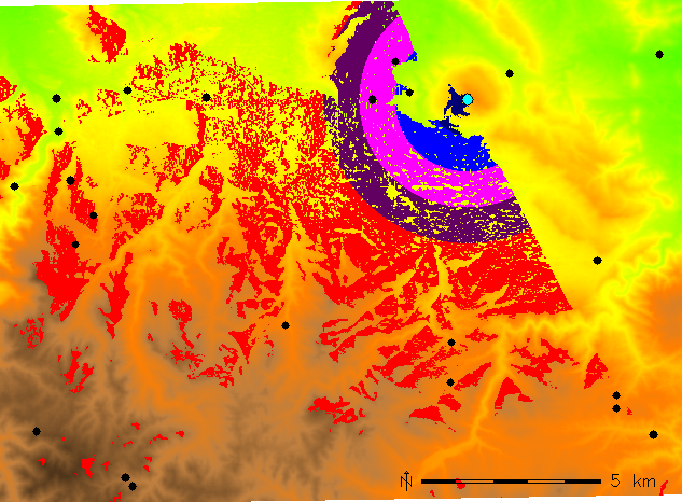
\includegraphics[width=0.7\textwidth]{visibility}
\captionof{figure}{Viewshed analysis efectuada com GRASS}
\end{myfig}

\section{Filosofia do Software livre}

O software livre garante ao utilizador o acesso ao c\'{o}digo fonte permitindo portanto transpar\^{e}ncia. Garante tamb\'{e}m o direito a estudar, extender alterar e redistribuir o mesmo c\'{o}digo, com o dever de ter de garantir os mesmos direitos aos outros utilizadores. A possibilidade de analise do c\'{o}digo fonte permite um processo de revis\~{a}o que garante a qualidade. Com a ajuda do extension manager \'{e} poss\'{i}vel criar novos m\'{o}dulos sem a necessidade de ter uma instala\c{c}\~{a}o completa de GRASS. 

\section{Ficha T\'{e}cnica}

\subsection{Licen\c{c}a}

General Public Licence (Free Software Foundation)

\subsection{Plataformas suportadas}

GRASS de facto funciona em qualquer plataforma, em particular com GNU/Linux, sistemas UNIX compat\'{i}veis com POSIX, MS-Windows e MacOS X.

\subsection{Estrutura}

\begin{itemize}
\item modular
\item mais de 350 m\'{o}dulos
\end{itemize}

\subsection{Linguagens de programa\c{c}\~{a}o}

\begin{itemize}
\item ANSI C
\item GRASS- SWIG interface
\item Python para aplica\c{c}\~{o}es WebGIS
\item Java: JGRASS
\end{itemize}

\subsection{Gest\~{a}o dos dados e potencialidades}

\begin{itemize}
\item processamento de dados Raster/Vectoriais/Voxel
\item modelos 2D/3D Raster e Vectoriais
\item elabora\c{c}\~{a}o de imagens
\item topologia vectorial e analise de redes
\item geoestat\'{i}stica (interface com R)
\end{itemize}

\begin{myfig}[1ex]
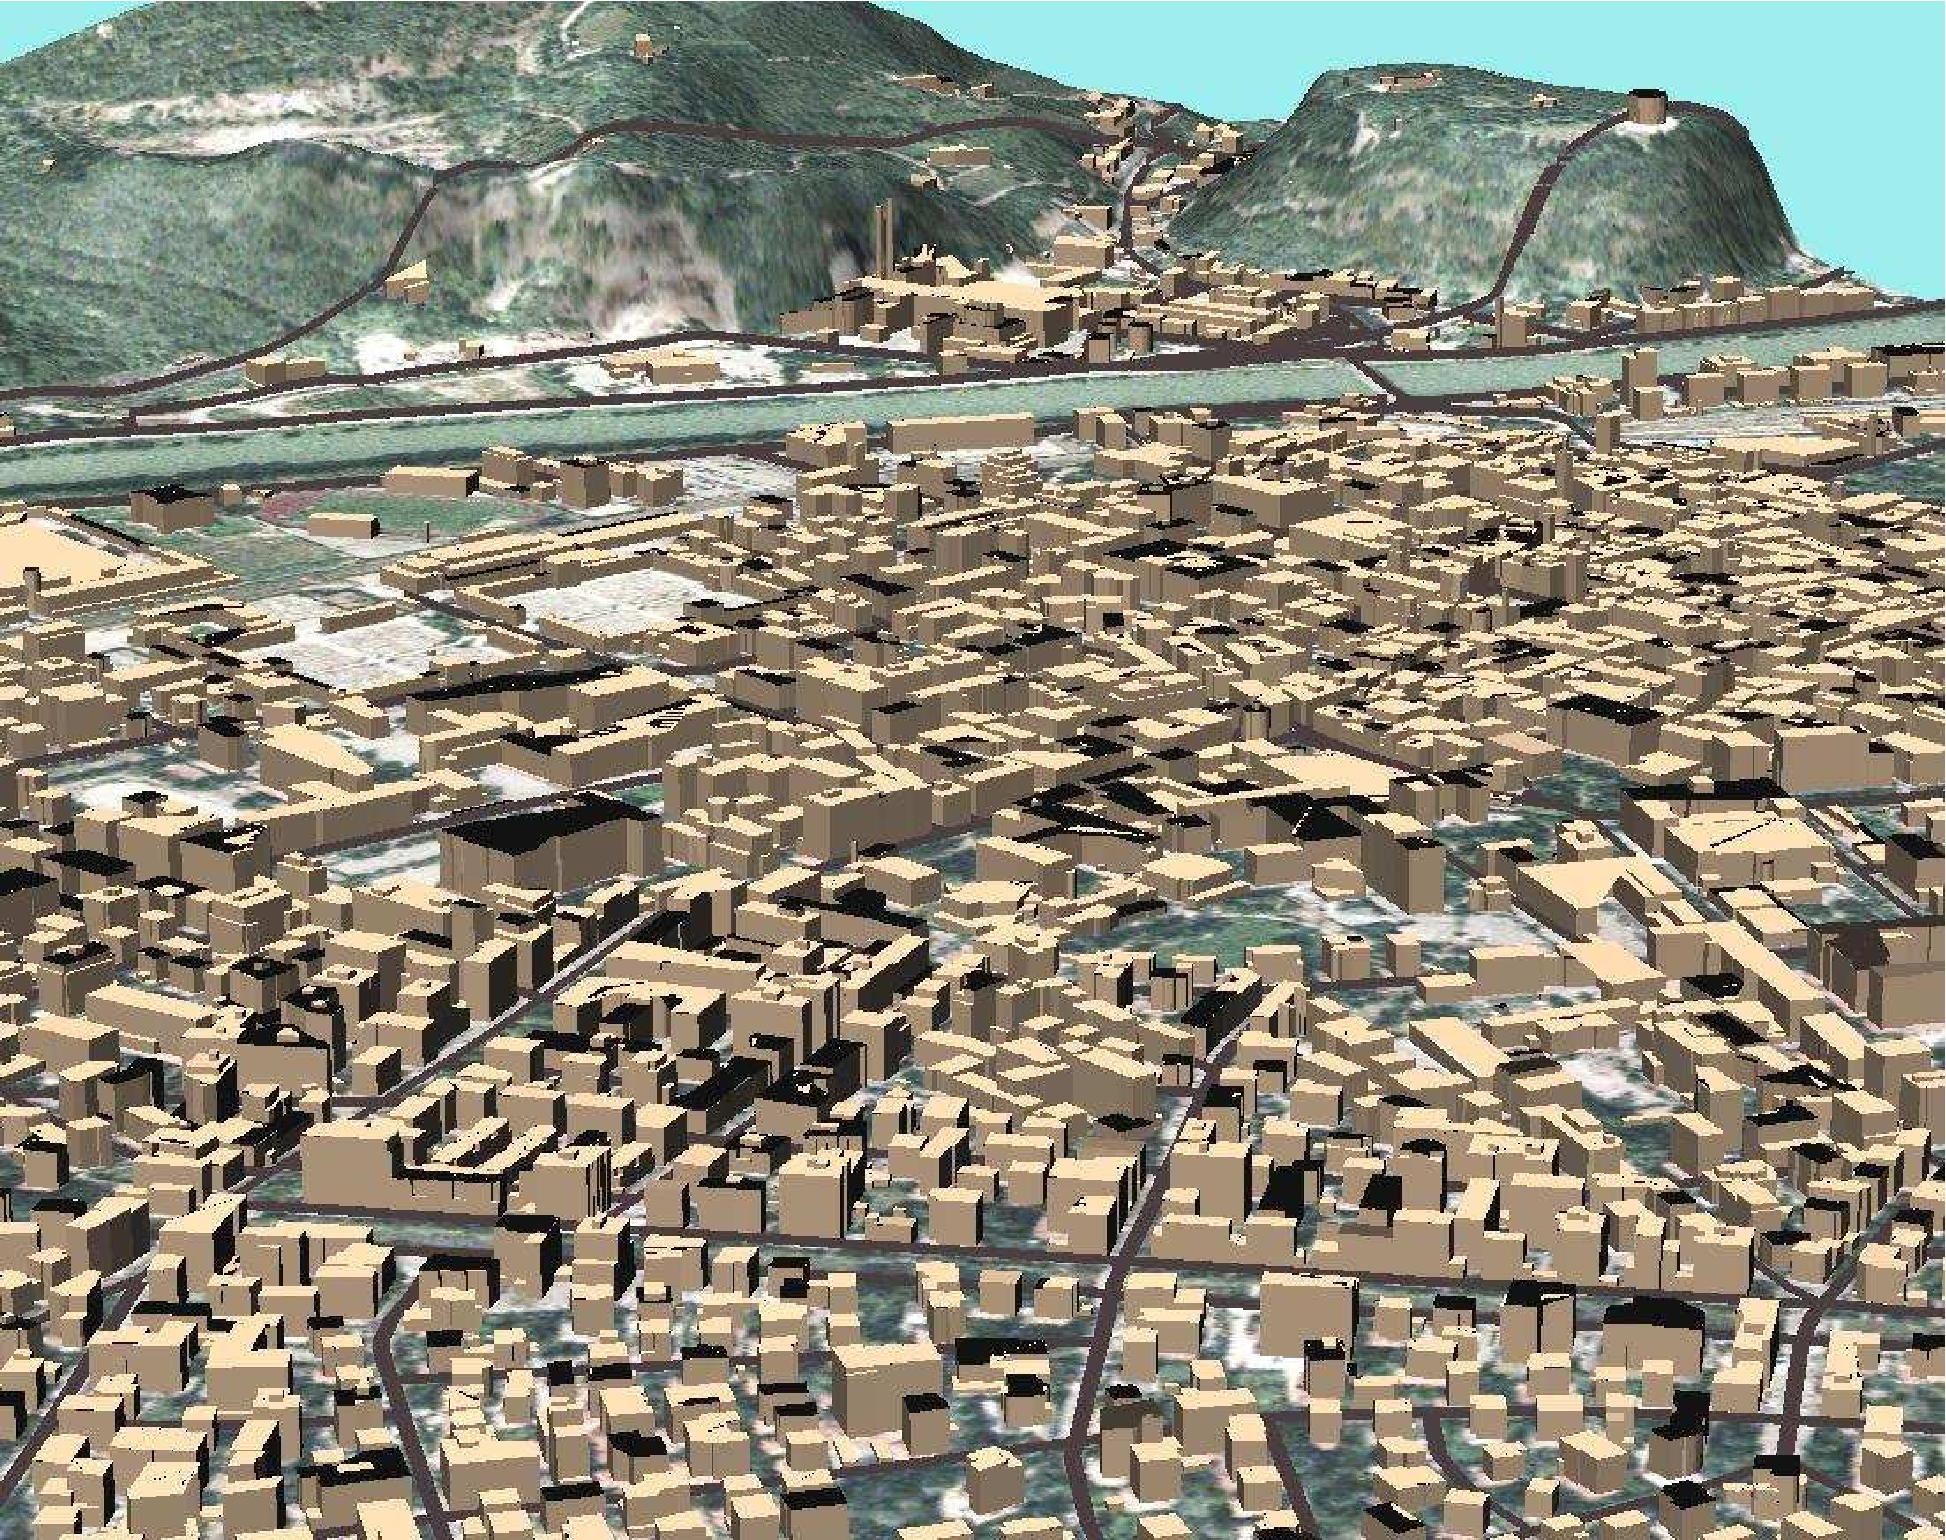
\includegraphics[width=0.7\textwidth]{trento3d}
\captionof{figure}{Vis\~{a}o a\'{e}rea da cidade de Trento (It\'{a}lia)}
\end{myfig}

\section{Formatos de ficheiros suportados}

GRASS fornece o suporte para todos os formatos de ficheiros SIG mais comuns atrav\'{e}s da utiliza\c{c}\~{a}o do package GDAL/OGR. Suporta ainda o standard do Open GIS Consortium para as Simple Features.

\subsection{Formatos de ficheiros Vectoriais}
ASCII, ARC/INFO ungenerate, ARC/INFO E00, Arc\-View SHAPE, BIL, DLG (U.S.), DXF, DXF3D, GMT, GPS-ASCII USGS-DEM, IDRISI, MOSS, MapInfo MIF, PostGIS, TIGER, VRML, \dots

\subsection{Formatos de ficheiros Raster}
ASCII, ARC/GRID, E00, GIF, GMT, TIF, PNG, Vis5D, SURFER (.grd), \dots
\begin{myfig}
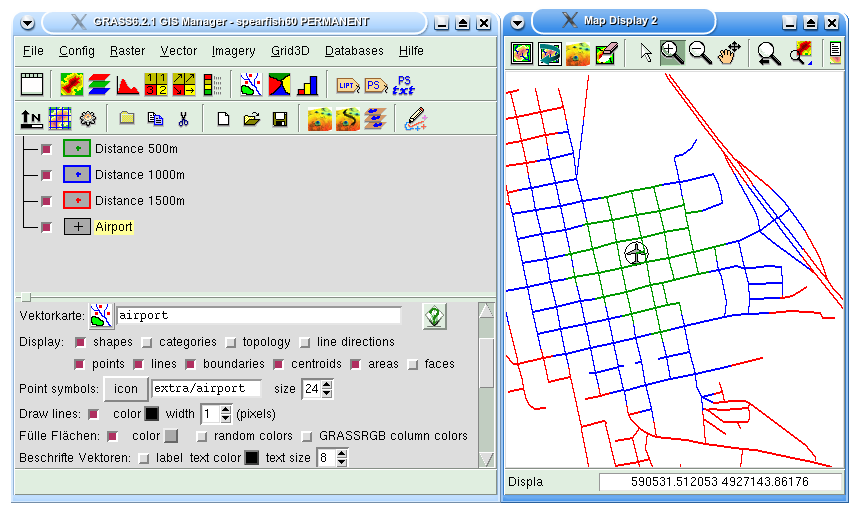
\includegraphics[width=0.7\textwidth]{isodist}
\captionof{figure}{Analise de redes atrav\'{e}s de interface gr\'{a}fica}
\end{myfig}

\subsection{Formatos de imagem}

CEOS (SAR, SRTM, LANDSAT7 etc.), ERDAS LAN / IMG, HDF, LANDSAT TM/MSS, NHAP aerial photos, SAR, SPOT, \dots
\begin{myfig}[1.5ex]
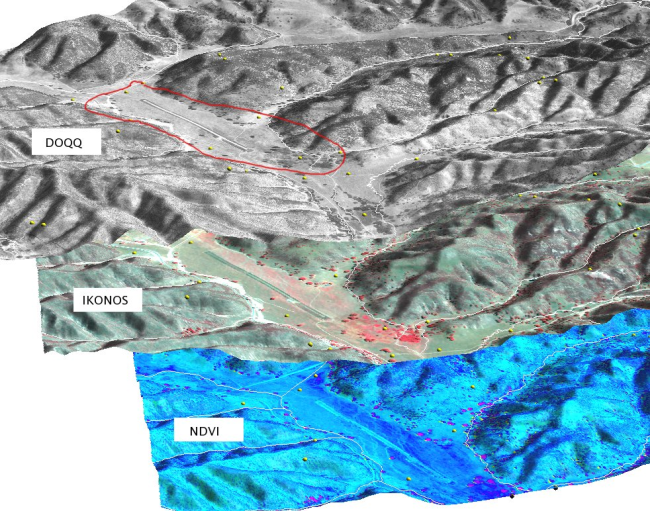
\includegraphics[width=0.7\textwidth]{ndvi}
\captionof{figure}{An\'{a}lise de imagem com GRASS}
\end{myfig}

\subsection{Bases de Dados Suportadas}

\begin{itemize}
\item PostgreSQL / PostGIS
\item MySQL
\item SQLite
\item ODBC
\item DBF
\end{itemize}

\subsection{Output}

\begin{itemize}
\item M\'{o}dulos para a gera\c{c}\~{a}o de mapas
\item NVIZ para a visualiza\c{c}\~{a}o de dados 2.5D e 3D e cria\c{c}\~{a}o de imagens
%\item{GMT export}
%item{VRML}
\item VTK, POVray
\item WebGIS atrav\'{e}s Mapserver, Python, etc. 
\end{itemize}

\subsection{Intraoperabilidade com outros SIG e outros software}

\begin{itemize}
\item Quantum GIS (Visualiza\c{c}\~{a}o de geodados e outros)
\item R- Language (Estat\'{i}stica)
\item GGstat (Geoestat\'{i}stica)
\item UMN Mapserver (Webmapping)
\end{itemize}

\section{Onde encontrar informa\c{c}\~{o}es}

\begin{itemize}
%\begin{flushleft}
\item{S\'{i}tio web do projecto: \\\GRASSurl}
\item{GRASS Wiki: \\\url{http://grass.osgeo.org/wiki}}
\item{GRASS Promotion Team: \\\url{malte@perlomat.de}}
\item{GRASS mailing lists: \\\url{http://grass.osgeo.org/community/support.php}}
%\end{flushleft}
\end{itemize}

\vfill
\section{OSGeo}

GRASS \'{e} um projecto fundador da {\it Open Source Geospatial Foundation} a qual tem como objectivo criar softwares livres de elevada qualidade pela geociencia. Para mais informa\c{c}\~{o}es visite o site OSGeo:
\begin{center}

\includegraphics[width=0.8\textwidth]{OSGeo_logo}\\
\url{http://www.osgeo.org}
\end{center}

\end{document}
